\documentclass[12pt]{article}
\usepackage{latexsym}
\usepackage{epsfig}
\usepackage{amsmath}
\usepackage{amssymb}


\setlength{\topmargin}{0in}
\setlength{\leftmargin}{0in}
\setlength{\textwidth}{6in}
\setlength{\textheight}{9.5in}
\setlength{\parindent}{0.2in}
\setlength{\parskip}{.08in}
\voffset = -.45in
\hoffset = -.5in

\begin{document}

\newcommand{\lsp}[1]{\large\renewcommand{\baselinestretch}{#1}\normalsize}

\lsp{1}
\pagestyle{plain}
\begin{center}
{\bf
Kruskal Worksheet
}
\end{center}

\begin{figure}[h]
\center
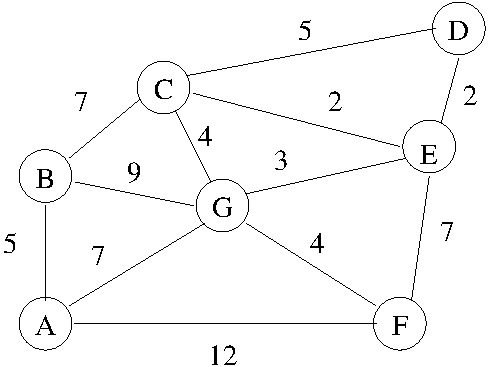
\includegraphics[width = 3in]{spanning.pdf}
\end{figure}

\begin{enumerate}
\item List the edges in non-decreasing order of weight.

\begin{tabular}{|c|c|c|c|c|c|c|c|c|c|c|c|} \hline
~~$E_1$ & ~~$E_2$ & ~~$E_3$ & ~~$E_4$ & ~~$E_5$ & ~~$E_6$ & ~~$E_7$ & ~~$E_8$ & ~~$E_9$ & ~~$E_{10}$ & ~~$E_{11}$ & ~~$E_{12}$ \\ \hline
 & & & & & & & & & & & \\ 
 & & & & & & & & & & & \\ \hline 
\end{tabular}

\item Start with spanning tree $T = \{ \}$. For each edge in order, 
check whether it creates a cycle? If not, add it to $T$.

\begin{tabular}{|l|c|} \hline
Edge  & Cycle?\\ \hline
$E_1$ & \\ \hline
$E_2$  & \\ \hline
$E_3$ & \\ \hline
$E_4$ & \\ \hline
$E_5$ & \\ \hline
$E_6$ & \\ \hline
$E_7$ & \\ \hline
$E_8$ & \\ \hline
$E_9$ & \\ \hline
$E_{10}$ & \\ \hline
$E_{11}$ & \\ \hline
$E_{12}$ & \\ \hline
\end{tabular}

\end{enumerate}
\end{document}
